\section{Introduction}
\label{intro}

There are no restrictions on which national jurisdictions BGP paths must or must not cross.  There is also no way for an Internet user to know or decide which countries her Internet traffic is transitting.  Internet routing is usually studied at the AS (Autonomous System) level - not the nation-state level.  An AS typically controls traffic as it transits it's internal network and then defines policies for filtering, monitoring, and routing traffic to the next AS.  It is becoming increasingly common for governments to require certain actions of ASes, such as enabling wiretapping or performing censorship.  Once Internet traffic enters a country, it is subject to that country's requirements, and subsequently the corresponding ASes' actions.  More and more countries are either trying or have already passed laws that allow for mass surveillance on their citizens~\cite{france_surveillance, netherlands_surveillance, kazak_surveillance}.  Recently, the Investigatory Powers Bill (IP Bill) in the UK, if passed, will require ISPs to store citizens' browsing history for a year, and allow intelligence agencies to collect bulk data on their citizens~\cite{uk_bill}.

Currently, governments are becoming more suspicious about where their citizens' traffic is going, and are facing the challenge of controlling which countries transit the traffic.  Governments and users have been motivated more than ever since the Snowden revelations to avoid countries known for surveillance practices, specifically the United States~\cite{russia_secure_internet, routing_errors, dte}.  More recently, the Safe Harbour agreement, an agreement that allows the free flow of data between the US and the EU, was struck down because it would give the NSA access to EU citizens' personal data~\cite{safe_harbour_illegal, safe_harbour_undecided}.

In response to the Snowden revelations, Brazil has taken great measures to avoid Internet traffic from being wiretapped by the NSA~\cite{brazil_history, brazil_break_from_US, brazil_conference, brazil_conference2, brazil_human_rights}.  Some of the actions that have been taken to avoid NSA surveillance include: building a 3,500 mile long fiber-optic cable from Fortaleza to Portugal (with no use of American vendors), pressing companies such as Google, Facebook, and Twitter (among others) to store data locally, switching its dominant email system (Microsoft Outlook) to a state-developed system called Expresso~\cite{brazil_cable, brazil_us_companies}.  In other efforts, Brazil has been building Internet eXchange Points, which help grow Internet connectivity and performance~\cite{brazil_IXP1, brazil_IXP2}; it also allows them to increase their connectivity with many other countries.  Brazil now has the largest national ecosystem of public Internet eXchange points in the world~\cite{brazil_ixp_ecosystem}.  It has also been shown that over the past few years, the number of ASes in Brazil that are connected internationally have grown significantly~\cite{brazil_international_ases}.  The case of Brazil shows that countries, governments, and Internet users are motivated to avoid surveillance conducted by other countries.

Determining which countries transit Internet traffic, which countries host the only server for a given domain, and which countries are avoidable for a given domain are challenging problems.  The first challeng arises from determining the country-level path that traffic takes; paths can be collected from either the data-plane - IP-level paths - or the control-plane - AS-level paths.  Our work uses the data-plane to analyze traffic paths; in order to determine which countries are on the path, the IP-level path must be mapped to a country-level path.  This is challenging because there is no ground truth for geolocation data; there is no guarantee of accuracy or completeness.  To address this challenge, we use different geolocation tools to increase our confidence in the country-level paths we collect.  More challenges arise in determining how to avoid countries; websites are complex and can fetch data from multiple third parties, which are likely located in different geographic locations, and therefore cross different countries' borders.  The increased usage of anycast IP complicates country avoidance because it gives clients less information about the location of the server from which they are accessing content.  

In this paper, we first shed light on how much traffic is currently transiting countries known for surveillance, with a focus on the US.  Despite the measures taken by different countries to avoid the US, we still see Internet traffic that transits the US.  We conduct a measurement study that helps quantify the existing possibilities for state-sponsored surveillance.  We take Brazil as a case study, and analyze the country-level paths from machines in Brazil to the Brazil Alexa Top 100 domains.  Knowing that Brazil has taken actions to avoid traffic transitting the US, we measure how much traffic is solely transitting the US, and how much traffic is destined for the US.  These are two distinct scenarios.  If the US is solely a country on the path (and not the end point), then there is the possibility for avoiding the US.  If the domain is solely hosted in the US, and therefore destined for the US, then the US cannot be avoided for the given domain.  Using RIPE Atlas probes and the Digital Envoy geolocation service, we find that out of 36,833 traffic paths originating in Brazil to the Brazilian Alexa Top 100 domains, 2,699 are solely transitting the US and the US is the destination for 28,196 of them (this does not necessarily mean that the US is the only possible destination, but it is the destination for Brazilian Internet users)~\cite{ripe_atlas, digital_envoy}.  

Next, we present and implement a new system for surveillance circumvention for Internet users, which finally gives the users some control over where their traffic is flowing.  Because popular web companies are opening or expanding their datacenters in Europe, there are more possible paths to get data~\cite{eu_datacenters}.  It is possible that a path from a client in Brazil to a datacenter in Europe does not pass through any country known for surveillance, but may be a longer path than the best path to a datacenter in the US, as shown in Figure~\ref{fig:intro}.  Our system leverages a geographically diverse set of relay machines that act as proxies to access data from servers located in different geographic regions.  A client will first query an oracle for the best relay to use in order to avoid a given country.  Then the oracle will respond with the IP address of the best relay, which the client will then send it's request to.  The relay will fetch the data from the domain's closest server and return the data to the client. \annie{Add a couple highlights of the results/evaluation section when we get there.}

\begin{figure}
\centering
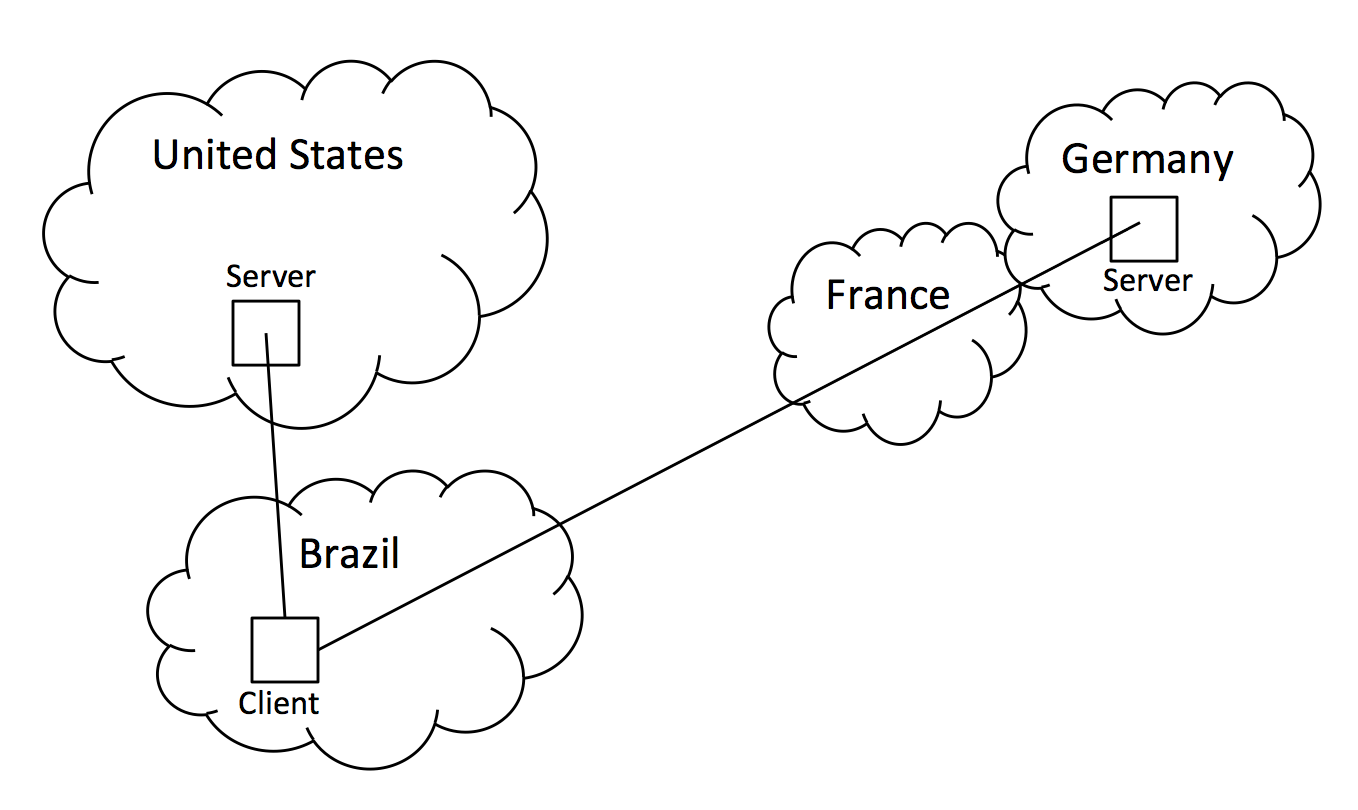
\includegraphics[width=.5\textwidth]{intro_fig}
\caption{A shorter path to a server in a country known for surveillance (U.S.), and a longer path to a georeplicated server in Germany.  The longer path may be more preferred by the client because it doesn't traverse a country with known surveillance practices.}
\label{fig:intro}
\end{figure}

This paper is organized as follows.  In the next section, we describe our research goals, and the challenges in achieving them.  In Section~\ref{datasets} we discuss how and where we collected our data.  We point out the advantages and disadvantages of existing datasets, and justify our decision.  In Section \ref{measure}, we design and execute a measurement study on the country-level paths of Brazil's Internet.  We describe our methodology, as well as results that show which countries Brazil's Internet traffic is traversing.  Next, Section \ref{architecture} introduces SYSTEM, which allows Internet users, ISPs, and Internet services to avoid specified countries, and therefore circumvent surveillance.  Then we explain our implementation of SYSTEM in Section \ref{implementation}.  In Section \ref{evaluation}, we evaluate our system and proposed methods for how well they avoid any given country.  We discuss how our system differs from others and uniquely suits the purpose of country avoidance in Section \ref{discussion}, we review related work in Section \ref{related}, and conclude in Section \ref{conclusion}.
